\section*{Question \#4B}

I knew something was wrong here, this is why I started writing down the domain and ranges of the functions (in problems A to C).

In my case, I defaulted to thinking that $\left(f^{-1} \circ f \right)\left(x\right) = x$, which is only true for $0 \leq x \leq \pi$ (which is a really dumb mistake in hindsight).

\begin{figure}[!h]
\definecolor{linecolor}{HTML}{0074C8}
\providecommand{\ival}[2]{\lbrack #1,#2 \rbrack}
\begin{tikzpicture}[scale=1.2,every node/.style={font=\small}]
\begin{scope}[dashed,line width=1pt,x=6cm/360]
\draw[black!60,solid,line width=0.3pt,-latex] (-110,0) -- (290,0) node[right] {$x$};
\draw[black!60,solid,line width=0.3pt,-latex] (0,-1.5) -- (0,1.5) node[above] {$y$};
\pgfplothandlerlineto
\pgfplotfunction{\x}{-90,-85,...,270}{\pgfpointxy{\x}{cos(\x)}}
\pgfusepath{stroke}
\node[black,below right] at (0,0) {$0$};
\foreach \pos in {-90,90,180,270}
\draw[black!60,line width=0.3pt,solid,shift={(\pos,0)}] (0pt,3pt) -- (0pt,-3pt);
\foreach \pos in {-1,1}
\draw[black!60,line width=0.3pt,solid,shift={(0,\pos)}] (3pt,0pt) -- (-3pt,0pt)
    node[black,left] {$\pos$};
\node[black,below] at (90,-0.1) {$\tfrac{\tau}{4}$};
\node[black,below] at (180,-0.1) {$\tfrac{\tau}{2}$};
\node[black,below] at (-90,-0.1) {$-\tfrac{\tau}{4}$};
\node[black,below] at (270,-0.1) {$\tfrac{3\tau}{4}$};
\node[black,above] at (90,1) {$y=\cos\;x$};
\end{scope}
\begin{scope}[color=linecolor,line width=1.5pt,x=6cm/360]
\pgfplothandlerlineto
\pgfplotfunction{\x}{0,5,...,180}{\pgfpointxy{\x}{cos(\x)}}
\pgfusepath{stroke}
\fill (0,1) circle (2pt);
\fill (180,-1) circle (2pt);
\end{scope}
\end{tikzpicture}\vspace{-6mm}
\end{figure}

\newpage

Anyway the following is what I should have written: 

\newcommand{\Comp}[3]{\left({#1} \circ {#2} \right)\left( {#3} \right)}
\newcommand{\Cos}[1]{\cos \left( {#1} \right)}
\newcommand{\Sin}[1]{\sin \left( {#1} \right)}
\newcommand{\Arccos}[1]{\arccos \left( {#1} \right)}

Given $\Comp{\arccos}{\cos}{\frac{7}{4}\pi}$:

\begin{equation}
\begin{split}
    \Cos{\frac{7}{4}\pi} &= \Cos{\frac{14}{8}\pi} \\
        &= \Cos{\pi + \frac{6}{8}\pi} \\
        &= \Cos{\pi}\Cos{\frac{6}{8}\pi} - \Sin{\pi}\Sin{\frac{6}{8}\pi} \\
        &= (-1)\left(-\frac{\sqrt{2}}{2} \right) - 0\Sin{\frac{6}{8}\pi} \\
        &= \frac{\sqrt{2}}{2} \\
        &= \alpha
\end{split}
\end{equation}

Therefore, we now consider $\Arccos{\alpha}$, which is a special angle and therefore easy to identify (in my case I memorized the special angles in terms of fractions of a circle):
\begin{equation}
\begin{split}
    \Arccos{\alpha} &= \Arccos{\frac{\sqrt{2}}{2}} \\
        &= \frac{1}{8}\tau \\
        &= \frac{1}{4}\pi
\end{split}
\end{equation}

Therefore:

\begin{equation}
\begin{split}
    \Comp{\arccos}{\cos}{\frac{7}{4}\pi} &= \frac{1}{4}\pi
\end{split}
\end{equation}

\section*{Regarding better studying habits}

Overall, I should really do \textbf{all} of the practice problems (at least some from each topic). Although this applies more to my calculus class (e.g. I was pretty confident about a topic, and therefore I didn't bother to review the associated practice material, which has happened on two occasions, and in both, there was something weird that tripped me up.)


\section*{Miscellaneous}

Regarding the remark that fractions are our friends, this was because it was evaluated VIA a calculator, which I punched in as fast as I could. What happened is that in a few places, I happen to use the same variable names as in the given formulas, and therefore got a few symbols mixed up (i.e. in one place, $\alpha$ should have been $\beta$ and vice-versa.). After I realized my mistake, I recomputed the answers as fast as I could. 



